\documentclass{standalone}
\usepackage{standalone}

\begin{document}
\chapter{Experiments}
\label{chap:experiments}
We have run several experiments based on the initial models keeping some properties basic like: 
\begin{itemize}
    \item Basic features for training
    \item Generating all set and get the best answer
\end{itemize}

We have experimented with:
\begin{itemize}
    \item Different neural network architecture
    \item Class differences for feature
    \item Choosing higher probabilistic tags for tagging. 
\end{itemize}
We have divided our dataset into 80:20 for training and test set. The training set contains 3461 lines and the test set contains 1483 lines. We have also processed the training lines suitable for our training features. For each word, we have created a line containing the probabilistic feature of it’s previous and next two words and it’s own feature. An example is shown in figure \ref{trainset}

\section{Initial Model}
We have conducted our first experiment exactly based on the model described in section \ref{train} and \ref{tagging}. We have got an accuracy of only \textbf{51.71\%.} An example is shown in figure \ref{exp1}.
 \begin{figure}[h!]
    \centering
    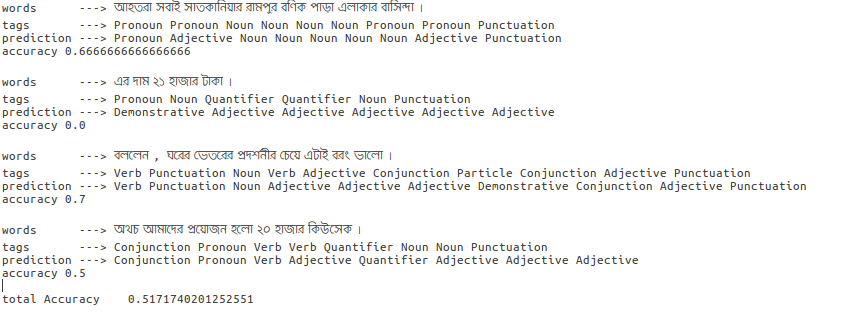
\includegraphics[width=1.0\columnwidth]{img/exp1.png}
    \caption{Initial model tags example}
    \label{exp1}
\end{figure}
\subsection{Drawbacks}
From the initial model, we can see some major drawbacks :
\begin{itemize}
    \item As we have discussed our tagging process in section \ref{tagging}, we are generating all possible combinations and then taking the one with minimum error score as the result. But there can be some cases where error score can be the same for multiple combinations. We did not handle this case so the program was picking the first best combination as a result. That is not a good idea to implement.
    \item As discussed in section \ref{feature} while calculating feature we are adding the probability to the corresponding class value. Where class values are 1,2...12. The difference between the two consecutive class values is only 1. So let for a word, the probability of being class 1 is 0.99999 and for class 2 it is 0.000001 so we will get the feature as 1.99999 and 2.000001 both are very close to each other. So they may create a problem for some models.
\end{itemize}
\subsection{modifications}
In order to recover the drawbacks discussed, we have decided to run further experiments with some modifications.
\begin{itemize}
    \item \textbf{High Probability First :} In case of the same error score for different combinations, we will take the one with the highest probability. For a combination of words and tags  ( word$_1$ , tag$_1$ ), ( word$_2$ , tag$_2$ ) ... ( word$_n$ , tag$_n$ ) the probability of being that combination a good one is product of the probabilities P(word$_i$ , tag$_i$ ). That means we will take the maximum of $\prod_{i=1}^{len(sentence)} P(word_i , tag_i)$.This technique theoretically  increases the chance of getting the best tags.
    
    \item \textbf{Higher Class Differnce :} For the second drawback, we would increase the class difference by 1 that is the class scores will be now 2,4,6...12. That decreases the chance of two different tags getting the same value. 
\end{itemize}
\subsection{Experiments Results}
We have conducted three different experiments on the initial model. first without any modification, then adding the high probability first and then with a higher class difference. The result is shown in the table \ref{inittable}

    \begin{table}[h!]
    \centering
        \begin{tabular}{|c|c|}
            \hline
            \textbf{model} & ]\textbf{accuracy} \\ [1ex]
            \hline
            initial model & 51.71\% \\
            \hline
            initial model + Higher Probability First & 72.9\%\\
            \hline
            initial model + Higher Probability First + Higher Class
            Difference & 84.7\%  \\ 
            \hline
        \end{tabular}
        \caption{experiment results with initial model}
        \label{inittable}
    \end{table}
\section{Multilayer Architecture}
We have conducted some more experiments with keeping every other thing unchanged except the neural network. We introduced the modern multilayer neural network architectures. 
\subsection{Sequential Model} We have used Keras Sequential model\cite{Charles2013} to build our multilayer Architecture for training purposes. Sequential is the easiest way to build a model layer by layer. We have experimented on 2 different architectures. We have got 82
\begin{itemize}
    \item Our first network is described in figure \ref{arc1}. We have run two tests, one with Higher Class Difference and another without it. We have kept Higher Probability First in both the experiments. The number of iteration in this network was only 100.

        \begin{figure}[h!]
        \centering
        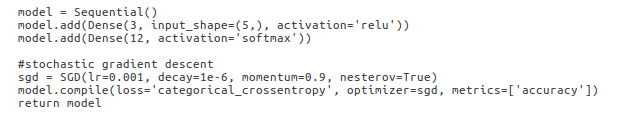
\includegraphics[width=1.0\columnwidth]{img/model1.png}
        \caption{Sequential model Architecture 1}
        \label{arc1}
        \end{figure}
        We have got 82.7\% without Higher Class Difference and 89.3\% with it. The result is shown in table \ref{res2}
        \begin{table}[h!]
        \centering
        \begin{tabular}{|c|c|}
            \hline
            \textbf{model} & ]\textbf{accuracy} \\ [1ex]
            \hline
            Sequential model + Higher Probability First & 82.7\%\\
            \hline
            Sequential model + Higher Probability First + Higher Class
            Difference & 89.3\%  \\ 
            \hline
        \end{tabular}
        \caption{experiment results with Sequential model Architecture 1}
        \label{res2}
    \end{table}
    \item Our Second network is described in figure \ref{arc2}. The differences from the earlier network are that it has 5 dense layers and iteration is increased to 1000. We have run two tests, one with Higher Class Difference and another without it. We have kept Higher Probability First in both the experiments. 

        \begin{figure}[h!]
        \centering
        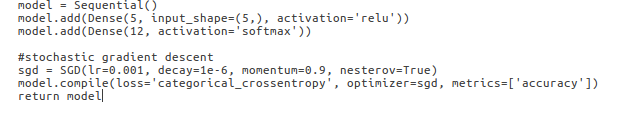
\includegraphics[width=1.0\columnwidth]{img/model2.png}
        \caption{Sequential model Architecture 2}
        \label{arc2}
        \end{figure}
        We have got 83.8\% without Higher Class Difference and 89.45\% with it. The result is shown in table \ref{res3}
        \begin{table}[h!]
        \centering
         \begin{tabular}{|c|c|}
            \hline
            \textbf{model} & ]\textbf{accuracy} \\ [1ex]
            \hline
            Sequential model + Higher Probability First & 83.8\%\\
            \hline
            Sequential model + Higher Probability First + Higher Class
            Difference & 89.45\%  \\ 
            \hline
        \end{tabular}
        \caption{experiment results with Sequential model Architecture 2}
        \label{res3}
        \end{table}
\end{itemize}

\section{Bidirectional LSTM}
LSTM (long short-term memory) is a novel, gradient-based method for sequence labeling\cite{doi:10.1162/neco.1997.9.8.1735}. LSTM has been used for POS Tagging in different languages\cite{ma2016endtoend}\cite{huang2015bidirectional}\cite{plank2016multilingual}\cite{wang2015unified}.We have used the Keras BiDirectional LSTM model. The model architecture is described in figure \ref{model3}. 
\begin{figure}[h!]
\centering
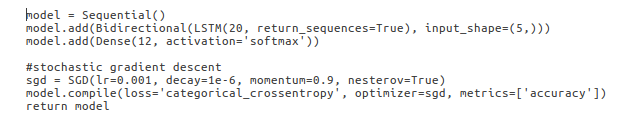
\includegraphics[width=1.0\columnwidth]{img/model3.png}
\caption{Bi-LSTM Network Architecture}
\label{model3}
\end{figure}

We have conducted three different tests on the model. The results have been shown in the table \ref{res4}
\begin{table}[h!]
        \centering
        \begin{tabular}{|c|c|}
            \hline
            \textbf{model} & ]\textbf{accuracy} \\ [1ex]
            \hline
            Bi-LSTM & 55.77\% \\
            \hline
            Bi-LSTM + Higher Probability First & 85.56\%\\
            \hline
            Bi-LSTM + Higher Probability First + Higher Class
            Difference & 90(89.98)\%  \\ 
            \hline
        \end{tabular}
        \caption{experiment results with Bi-Direcitional LSTM}
        \label{res4}
        \end{table}


\end{document}